\documentclass{article}[11pt]

\usepackage[french]{babel}
\usepackage[utf8]{inputenc}
\usepackage{color}
\usepackage{graphicx}
\usepackage{amsmath}
\usepackage{hyperref}

\begin{document}

\Large

\title{Projet robotique autonome :\\ \textbf{MLP Ball catcher}}

\author{Victor Cheimanoff, Thibaud Cheippe, Yoan Mollard}

\maketitle

\normalsize

\tableofcontents

\begin{figure}[!htc]
	\begin{center}
		
\includegraphics[scale=0.3]{images/logo_enseirb.png}
	\end{center}
\end{figure}

\newpage

\section{Introduction}

L'objet de ce projet est d'utiliser un bras robotique pour rattraper une balle qui lui serait lancée par un utilisateur. Le système utilise un équipement de motion tracking permettant de repérer la balle dans l'espace à l'aide de caméras. Une fois la trajectoire de la balle amorcée il calcule un point d'impact puis ordonne au bras de s'y positionner. \\

Bien que la main robotique soit capable de se fermer il semble important d'omettre ce détail dans un premier temps pour se consacrer sur l'obtention d'un impact entre la balle et le poignet. Ceci nottamment car orienter le bras dans une configuration où la balle peut rentrer au milieu des doigts ajout une difficulté supplémentaire. \\

Afin de conclure cette introduction nous présentons rapidement le matériel utilisé, à savoir le bras robotique et le système de capture Optitrack. L'ensemble de la scène est représenté en figure \ref{general}.

\subsection{Le bras robotique}

Le bras utilisé est un bras anthropomorphe à taille réelle conçu par Rhoban Project. Il dispose de sept servomoteurs Dynamixel immitant le bras humain. Il vient avec une suite logicielle conçue par l'équipe de Rhoban Project permettant de le manipuler, qui va consiter en trois éléments : \\

\begin{itemize}
\item Une interface graphique, RobotBoard, qui permet de créer et d'enregistrer des mouvements, que nous n'utiliserons pas dans ce projet. 
\item Le RhobanServer qui gère la communication bas niveau avec le matériel
\item Le SDK Rhoban, qui nous permet d'envoyer des instructions au robot, ainsi que de lire facilement les valeurs prises par les moteurs du robot, qui sera l'outil principalement utilisé pour notre projet.
\end{itemize}

\subsection{Le système de capture \og Motion tracking\fg}

Le système de capture utilisé est composé de trois caméras Optitrack VX1000. Equipées d'un éclairage infrarouge ces caméras, lorsqu'elles sont convenablement disposées autour d'une scène, permettent de localiser dans l'espace des boules réfléchissantes d'un centimètre de diamètre. Seuls les marqueurs réfléchissants fournis sont censés pouvoir être tracké par Optitrack. Cependant nous avons pensé à recouvrir notre balle de papier d'aluminium afin de substituer la balle aux marqueurs. \\

\begin{figure}[!htc]
	\begin{center}
		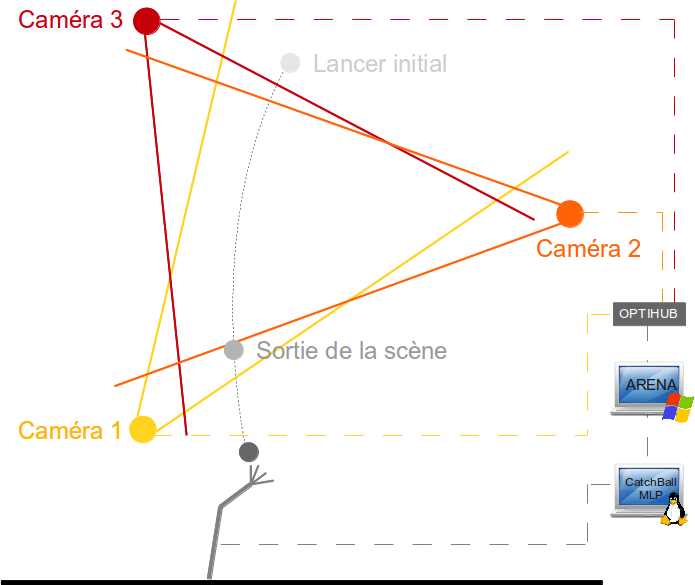
\includegraphics[scale=0.5]{images/general.png}
		\caption{Schéma de la scène : bras accompagné des trois caméras et leur champs de vision, balle et sa trajectoire, le serveur Windows sur lequel foncitonne Arena et auquel sont connectées les caméras et le client Linux composé de trois modules et pilotant directement le bras}
		\label{general}
	\end{center}
\end{figure}

\section{Découpage du projet}

Nous avons décomposé le projet en trois parties distinctes :
\begin{itemize}
\item La mise en place du système de capture Optitrack de manière à obtenir les coordonnées x, y, z d'un point de l'espace
\item L'obtention du modèle géométrique inverse du robot, le calcul de la trajectoire de la balle et la planification du point d'impact
\item La représentation 3D (OpenGL) de la scène pour visualiser la trajectoire calculée, le point d'impact choisi et éventuellement la configuration du robot \\
\end{itemize}

\subsection{Trois exécutables distincts}

L'idée est de conserver ces trois parties indépendantes dans trois exécutables différents, puis de les faire communiquer sur leurs entrées et sorties standard en utilisant un protocole texte très simple. Les trois exécutables sont :
\begin{itemize}
\item Le client récupérant les coordonnées diffusées par Arena (Client/Data Streaming)
\item Le calculateur de la trajectoire de la balle planifiant le point d'impact (Impact)
\item L'affichage en temps réel (Viewer) \\
\end{itemize}

Ce découpage est représenté sur la figure \ref{general}. On lance ainsi le programme final en redirigeant les sorties au bon exécutable :
\begin{verbatim}
~$ ./Client | ./Impact | ./Viewer
\end{verbatim}

\begin{figure}[!htc]
	\begin{center}
		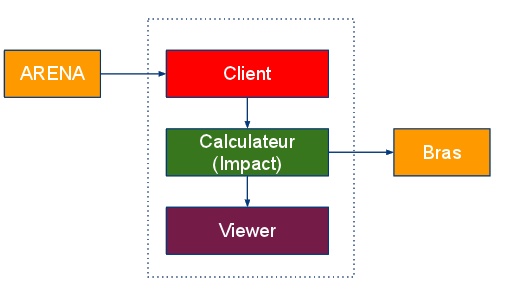
\includegraphics[scale=0.5]{images/tout.png}
		\caption{Découpage de l'application en trois modules : données Arena en entrée et commande du robot en sortie} 
		\label{general}
	\end{center}
\end{figure}

\subsection{Le protocole}

Il est nécessaire de définir un protocole basique de communication entre les trois exécutables. Bien qu'il n'ait pas encore été spécifié, voici un exemple de ce qui pourrait être utilisé : \\
\begin{itemize}
\item Entre le client et le calculateur, on transmet pour chaque instant t les coordonnées x, y, z de la balle dans le repère de la scène sur une nouvelle ligne : \\
\begin{verbatim}
t      x      y      z
\end{verbatim}
Par exemple :
\begin{verbatim}
0.01   45.3   24.8   176.4
0.02   45.9   23.9   174.2
0.03   47.5   24.1   171.7
0.04   51.0   23.2   167.9
...    ...    ...    ...
\end{verbatim}

\item
\item Entre le calculateur et le visualisateur, on inclue les précédents relevés $t, x, y, z$ de position de la balle ainsi que les paramètres de trajectoires $A_x$, $A_y$, $A_z$, $B_x$, $B_y$, $B_z$. On identifie une trajectoire grâce à un entier "id" pour pouvoir aisément la mettre à jour lors de l'obtention d'un nouveau point :
\begin{verbatim}
t       x      y      z
id      ax     ay     az     bx     by     bz      // Mise à jour ou création
                                                   // de la trajectoire numéro "id"
\end{verbatim}
Par exemple :
\begin{verbatim}
0.01   45.3   24.8   176.4
0.02   45.9   23.9   174.2
0.03   47.5   24.1   171.7
0.04   51.0   23.2   167.9
1      18.6   34.8   44.9    33.12  178.6  8.7    // Création de la trajectoire 1
0.05   42."   24.9   170.3
0.06   51.7   23.4   167.2
1      17.6   34.8   44.9    33.12  178.6  8.7    // Mise à jour de la trajectoire 1
0.07   49.9   23.9   176.2
\end{verbatim}
\end{itemize}

\section{Exportation des coordonnées d'un point avec Optitrack}

Cette partie est un tutoriel de mise en route rapide du système de capture, principalement à destination des futurs utilisateurs ou repreneurs du projet. Le fabriquant du système documente peu ses produits mais les tutoriels sont plutôt utiles \cite{naturalpoint_tutoriels}. \\

La première étape consiste à disposer les caméras autour de la scène. Six caméras sont fournies dans le pack, mais nous avons commencé par en monter seulement trois sur trépied. Selon la qualité des résultats obtenus il est possible d'ajouter des trois autres à mi-hauteur sur les trépieds pour augmenter la précision des coordonnées obtenus. \\

Les trois (ou les six) caméras sont connectées à un hub USB (Optihub) lui-même connecté à un PC sur lequel est installé le logiciel Arena. Il est important de disposer les caméras plutôt vers le début de la trajectoire de la balle, car c'est ici qu'il nous reste suffisamment de temps pour effectuer les calculs et surtout positionner le bras robot à la position calculée. \\

\subsection{Calibration des caméras}

La première étape consiste à calibrer les caméras entre elles. En démarrant l'utilitaire de calibration d'Arena on commence par jouer sur les paramètres ainsi que sur l'orientation des caméras. Selon nos essais, il est préférable d'éviter que les caméras se voient les-unes-les-autres et de choisir une intensité faible pour les LEDs infrarouge : une trop forte intensité augmente le nombre de parasites. Avant de continuer il faut s'assurer qu'aucun point parasite n'est détecté par l'une des caméras en l'abscence de marqueur dans la scène. Les parasites peuvent être des objets réfléchissants ou brillants (fenêtre, lumière, métal ...). Afin de comprendre d'où proviennent les parasites il est utile d'afficher les images noir et blanc renvoyées par les caméras (clic droit sur une frame puis Grayscale image). Avant de commencer la calibration aucun parasite ne doit apparaître en l'absence de marqueur et un marqueur placé dans la scène doit être reconnu par les trois caméras. \\

L'étape de calibration peut ensuite commencer. Il s'agit de déplacer trois marqueurs au bout d'une baguette Optiwand pour couvrir au maximum le volume de la scène dans un maximum d'orientations possibles. Toutes les caméras doivent visualiser les marqueurs pour que les points puissent participer à la calibration. A l'issue du processus de calcul Arena est capable de disposer les caméras dans l'espace les unes par rapport aux autres sur une carte. 
\newpage
<<<<<<< HEAD
Il faut ensuite placer le repère (représenté par une équerre en métal sur laquelle sont disposés trois marqueurs) afin de définir l'origine et l'orientation des axes du repère.\\
=======
Il faut ensuite placer le repère (représenté par une équerre en métal sur laquelle sont disposés trois marqueurs) afin de définir l'origine et l'orientation des axes du repère. La calibration est ainsi terminée et Arena peut afficher la position d'un marqueur dans l'espace.\\
>>>>>>> 30c2422cf352727868de7aa5bca667e4d0f973c8

Note : la licence Arena a été enregistrée pour la caméra 179282. Cette caméra doit donc impérativement être branchée pour démarrer Arena.

\subsection{Constitution d'un Corps Rigide}

<<<<<<< HEAD
Une fois les caméra calibrées, il est important de créer un corps rigide.
Un corps rigide représente un ensemble de points ne bougeant pas les uns par rapport aux autres. Cela nous permet de reconnaître facilement les points intéressant (comme les trois marqueurs de la baguette de calibration). De plus, il est impératif d'avoir un corps rigide afin de pouvoir transférer les positions à un programme tiers. La création d'un corps rigide se fait facilement en faisant bouger les marqueurs de l'objet dans le champs de vision des caméras.

\subsection{Exportation des coordonnées}

Arena embarque un serveur diffusant les coordonnées du corps rigide, apellé NatNet. Un client récupérant ces coordonnées existe déjà pour Windows, nous l'avons adapté pour qu'il puisse fonctionner sous Linux et pour l'intégrer à notre Ball catcher. 

\subsection{Calcul de l'erreur sur les coordonnées}
Afin de connaître la précision du système de motion tracking, nous avons mesuré l'écart entre deux marqueurs avec une règle, puis avec les coordonnées récupérées depuis le logiciel optitrack. En moyenne, on obtient une erreur de 3 millimètres tout les 25 centimètres 
\newpage
\section{Modélisation et Modèle Géométrique Inverse}
Nous désirons déplacer le robot en lui fournissant un position de destination absolue $(x, y, z)$ dans un repère lié à la salle. Or, le robot se positionne en utilisant les valeurs angulaires que doivent prendre ses moteurs. Il était donc nécessaire d'implémenter un module permettant de passer d'une position absolue aux valeurs angulaires associées, d'ou la nécessité du calcul d'un modèle géométrique inverse.

\subsection{Modelisation}




=======
Une fois les caméra calibrées, il est important de créer un corps rigide pusiqu'il s'agit a priori du seul moyen d'exporter les coordonnées des points capturés. \\

Un corps rigide représente un ensemble de points ne bougeant pas les uns par rapport aux autres. Cela nous permet de reconnaître facilement les points intéressants (comme les trois marqueurs de la baguette de calibration). De plus, il est impératif d'avoir un corps rigide afin de pouvoir transférer les positions à un programme tiers. La création d'un corps rigide se fait facilement en faisant bouger les marqueurs de l'objet dans le champs de vision des caméras.

\subsection{Exportation des coordonnées}

Arena embarque un serveur diffusant les coordonnées du corps rigide, apellé NatNet. Un client récupérant ces coordonnées existe déjà pour Windows, nous l'avons adapté pour qu'il puisse fonctionner sous Linux et pour l'intégrer à notre Ball catcher. Il correspond à la partie "Client" dans notre découpage.

\subsection{Calcul de l'erreur sur les coordonnées}
Afin de connaître la précision du système de motion tracking, nous avons mesuré l'écart entre deux marqueurs avec une règle, puis avec les coordonnées récupérées depuis le logiciel Arena. En moyenne, on obtient une erreur de 3 millimètres tous les 25 centimètres 
\newpage
\section{Modélisation et Modèle Géométrique Inverse}
Nous désirons déplacer le robot en lui fournissant un position de destination absolue $(x, y, z)$ dans un repère lié à la salle. Or, le robot se positionne en utilisant les valeurs angulaires que doivent prendre ses moteurs. Il était donc nécessaire d'implémenter un module permettant de passer d'une position absolue aux valeurs angulaires associées, d'ou la nécessité du calcul d'un modèle géométrique inverse.

\subsection{Modelisation}




>>>>>>> 30c2422cf352727868de7aa5bca667e4d0f973c8
\section{Prédiction de trajectoire}
Le module suivant est également intégré dans la partie "Calcul d'Impact", il permet de calculer et de prédire la trajectoire d'un projectile à partir des données relevées par le système Optitrack.

\subsection{Modèle physique}

Nous nous sommes placé dans le cadre de la mécanique Newtonienne, en considérant notre projectile comme un objet ponctuel, étant uniquement soumis à la force de gravitation terrestre, et en négligeant donc les forces frottements.\\

En considérant un repère orthonormé lié à la salle, dont l'axe z serait vertical, orienté vers le haut, nous avons donc ainsi des équations de trajectoire de la forme suivante :\\

$x = A_xt + B_x$\\

$y = A_yt + B_y$\\

$z = -\frac{1}{2} g t^2 + A_zt + B_z$\\

Ou les $A_i$ et $B_i$ sont des constantes d'intégration qui apparaissent lors du calcul de ces équations, et que nous cherchons donc à déterminer afin de prédire cette trajectoire.\\

Nous avons donc à ce niveau un système de trois équations à six inconnues, il nous faudra donc, d'un point de vue mathématique, et donc sans tenir compte des imprécisions du module de capture, les valeurs de positions du projectile à deux instants différents (ie : deux quadruplets $(x_i, y_i, z_i, t_i)$ ) afin de calculer les valeurs de ces constantes, et donc d'avoir l'équation de trajectoire du projectile.
\newpage
Avec deux tels quadruplets, nous obtenons les valeurs suivantes :\\

$A_x = \frac{x_j-x_i}{t_j-t_i}$\\

$A_y = \frac{y_j-y_i}{t_j-t_i}$\\

$A_z = \frac{(z_j + \frac{1}{2} g t_j^2)-(z_i + \frac{1}{2} g t_i^2)}{t_j-t_i}$\\

$B_x = x_i - A_x t_i$\\

$B_y = y_i - A_y t-i$\\

$B_z = z_i + \frac{1}{2} g t_i^2 - A_z t_i$\\

\subsection{Implémentation pratique}

Néanmoins, dans la pratique, les valeurs relevées par le module de motion tracking ne sont pas des valeurs exactes. Une imprécision dans la mesure, même faible, peut avoir des répercutions importantes sur les points éloignés d'une trajectoire qui serait modélisée à partir de ces seules mesures.\\

Afin de palier à ce problème, le module de prédiction de trajectoire va effectuer plusieurs calculs des solutions des équations de mouvements. Ceci à partir de différents quadruplets de points envoyés par le système de motion tracking. IL va également utiliser pour sa prédiction une moyenne arithmetique non pondérée sur les différentes valeurs ainsi calculées, ce qui nous permet de réduire l'erreur en augmentant le nombre de mesures. \\

Ainsi, en effectuant un nombre de mesure suffisant avec le système de motion tracking, nous devrions être en mesure d'obtenir une prédiction de trajectoire réaliste.
\newpage


\section{Représentation 3D de la scène, du bras, de la balle et de sa trajectoire}

Nous avons ajouté au projet un dernier module "visualisateur 3D" dont le rôle est de représenter la scène en 3D en temps réelle. Le minimum, et de loin le plus important est de représenter le système de coordonnées de la scène (défini par le Calibration Square), la trajectoire prévue et affinée à chaque instant, et le point d'impact calculé. \\

Le visualisateur utilise les bibilothèques OpenGL et GLUT pour QT. Les trois fichiers \textit{main}, \textit{window} et \textit{glwidget} s'occupent du fonctionnement global de l'application, de la fenêtre, et du composant OpenGL. Ils sont issus d'un exemple de QT pour OpenGL sous licence BSD. La scène est dessinée dans $GLWidget::paintGL()$, méthode appelée à chaque rafraichissement de l'image. Les éléments de la scène (balle, sol, mur, robot ...) sont déclarés dans l'en-tête de GLWidget et dessinés dans cette méthode $paintGL()$. Les éléments affichables sont :\\


\begin{itemize}
\item \textit{CoordinateSystem} : Cet élément représente le système de coordonnées de la scène. Il est déplacé en fonction du système de coordonnées OpenGL pour correspondre à celui réellement utilisé dans la scène.
\item \textit{Ball} : Cet élément représente une balle dont la couleur, le diamètre et la position dans l'espace sont moifiables
\item \textit{Plane} : Cet élément représente un plan, typiquement utilisé pour le sol et les murs. Il peut être dessiné soit avec un fond plein, soit avec un fond cadrillé et transparant
\item \textit{Arm} : Cet élément représente le bras, la position de la base et les angles des servomoteurs peuvent être modifiés. Le dessin fait appel au modèle géométrique. \\
\end{itemize}

Il est possible de déclarer autant d'exemplaires de bras, de balles ou de trajectoires que souhaité. Les trajectoires disposent d'un identifiant pour facilier leur mise à jour au cours du temps. \\

La figure \ref{viewer} est une capture du visualisateur, sur une scène comprenant un sol cadrillé, un mur gris plein, le repère scène à son pied à gauche (axe $x$ rouge, axe $y$ vert, axe $z$ bleu), ainsi qu'une trajectoire et une balle. Sur cette capture le bras n'est pas encore modélisé.
\begin{figure}[!htc]
	\begin{center}
		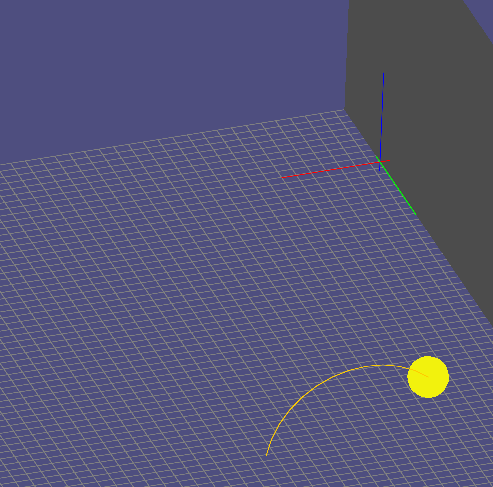
\includegraphics[scale=0.5]{images/viewer.png}
		\caption{Capture de la visualisation OpenGL d'un repère, un sol, un mur, une trajectoire et une balle} 
		\label{viewer}
	\end{center}
\end{figure}



\section{Conclusion}

Nous avons découpé ce projet en trois parties : l'obtention des coordonnées avec Arena, réalisée par le module "Client/Data streaming", le calcul de la trajectoire de la balle et du point d'impact réalisé par le module "Impact" qui commande le bras en faisant appel aux modèles géométriques direct et inverse du robot, et un visualisateur 3D permettant de représenter la scène. \\

Les trois parties ne sont pas encore terminées et demandent a être encore approfondies avant d'être rassemblées et qu'elle puissent communiquer ensemble grâce au protocole simple décrit dans ce rapport. L'utilisation obligatoire des marqueurs pour l'aquisition des points avec Optitrack nous empêche d'utiliser directement une balle. Même recouverte de papier aluminium les résultats ne sont pas satisfaisant, car plutôt que de détecter un point l'aluminium reflète plusieurs points qu'il est impossible de regrouper dans un corps rigide étant donné qu'il n'y en a pas toujours le même nombre. Une parade reste donc encore à trouver pour utiliser Optitrack avec une balle. \\

Faute de temps, l'implémentation du module de modélisation n'a pas pu être terminée. Néanmoins, nous disposons de tous les éléments nécessaires à son implémentation. Le visualisateur est pour l'instant capable d'afficher les principaux éléments graphiques, mais il ne s'agit que d'affichage. La source des données du visualisateur sont les autres modules : elles proviennent des informations transmises par Optitrack ou relayées/calculées par le calculateur de point d'impact. D'autre part la classe permettant de représenter le bras est pour le moment très incomplète, il lui faut s'appuyer sur le modèle géométrique direct pour dessiner correctement les seux segments représentant graphiquement le bras dans le modèle 3D.


\begin{thebibliography}{}
  \bibitem{naturalpoint_tutoriels}
  Tutoriels NaturalPoint Optitrack \\
  \url{http://www.naturalpoint.com/optitrack/products/arena/tutorials.html}

\end{thebibliography} 

\end{document}
